% !TeX program = lualatex
\documentclass[12pt, a5paper]{article}
\usepackage{fullpage}
\usepackage{subfiles}
\usepackage{fontspec}
\usepackage{libertine}
\usepackage{xcolor}
\usepackage{GotIn}
\usepackage{geometry}
\usepackage{multicol}
\usepackage{multicolrule}
\usepackage{graphicx}
\usepackage[autocompile]{gregoriotex}

\geometry{top=1cm, bottom=1cm, right=1cm, left=1cm}
\pagestyle{empty}

\definecolor{red}{HTML}{C70039}
% \input GoudyIn.fd
% \newcommand*\initfamily{\usefont{U}{GoudyIn}{xl}{n}}

\input Acorn.fd
\newcommand*\initfamily{\usefont{U}{Acorn}{xl}{n}}
% cette ligne ajoute de l'espace entre les portées
% \grechangedim{baselineskip}{60pt}{scalable}

\begin{document}
\gresetlinecolor{gregoriocolor}

\begin{titlepage}\centering
  \vspace*{\fill}\
  \huge Secondes Vêpres\\
  \large des dimanches ordinaires\\
  \medskip
  \large et\\
  \medskip
  \LARGE Salut du Saint-Sacrement
  \bigskip
  \begin{figure}[h!]
    \centering
    
\includegraphics[width=7cm]{logo.png}
  \end{figure}

  \vspace*{\fill}
  \large\textit{
    Livret latin-français
  }
\end{titlepage}

\begin{center}
  \rule{2cm}{0.4pt}
\end{center}

\vspace{5mm}
\begin{center}
  \textcolor{red}{\normalsize{Ouverture.}}
\end{center}

% greillumination: remplace la première lettre, ici par une font ornementale
\greillumination{\initfamily\fontsize{11mm}{11mm}\selectfont D}
\gregorioscore{vepres-deus_in_adjutorium}
\medskip

\begin{center}
  \small{
  \emph{
    Dieu, venez à mon aide ; Seigneur, hatez-vous de me secourir.\\
    Gloire au Père, au Fils et au Saint Esprit, comme il était au commencement, maintenant et toujour et dans les siècles des siècles.\\
    Ainsi soit-il. Alleluia.
  }
}
\end{center}


% \gregorioscore{vepres-deus_in_adjutorium_septuagesime}

% vfill : prends l'espace vertical disponible 
% 

% greseparator: ornement. Le premier parametre est le type (de 1 à 5), le second la taille en points
% \greseparator{4}{30}

\newpage

% ===== DEBUT Antienne =========
\greillumination{\initfamily\fontsize{11mm}{11mm}\selectfont D}
\gregorioscore{antiennes/dixit-dominus-domino-meo}
\begin{center}
  \footnotesize{
    \textit{
      L'Éternel a dit à mon Seigneur: Assieds-toi à ma droite.
    }
  }
\end{center}
\medskip
% ===== FIN Antienne ===========

% ===== DEBUT psaume ===========
% gresetinitiallines : avec le parametre à 0, supprime l'ornement
\gresetinitiallines{0}

\begin{center}
  \normalsize{Psaume 109.}\\
  \footnotesize{
    \emph{Génération éternelle du Christ, Prêtre, Roi et Juge.}
  }
\end{center}

\gregorioscore{psaumes/psaume109-VIIC2}
\begin{enumerate}
  \setcounter{enumi}{2}
  \item Virgam virtútis tuæ emíttet Dómi\textbf{nus} ex \textbf{Si}on:\textcolor{red}{~*} \\ \-\hspace{2cm} domináre in médio inimi\textbf{có}rum tu\textbf{ó}rum.

  \item Tecum princípium in die virtútis tuæ in splendóri\textbf{bus} sanc\textbf{tó}rum:\textcolor{red}{~*}\\ \-\hspace{2cm}  ex útero ante lucíferum \textbf{gé}nu\textbf{i} te.

  \item Jurávit Dóminus, et non pœni\textbf{té}bit \textbf{e}um:\textcolor{red}{~*}\\ \-\hspace{2cm}  Tu es sacérdos in ætérnum secúndum órdi\textbf{nem} Mel\textbf{chí}sedech.

  \item Dóminus a \textbf{dex}tris \textbf{tu}is,\textcolor{red}{~*} confrégit in die iræ \textbf{su}æ \textbf{re}ges.

  \item Judicábit in natiónibus, im\textbf{plé}bit ru\textbf{í}nas:\textcolor{red}{~*} 
  conquassábit cápita in \textbf{ter}ra mul\textbf{tó}rum.

  \item De torrénte in \textbf{vi}a \textbf{bi}bet:\textcolor{red}{~*} proptérea exal\textbf{tá}bit \textbf{ca}put.

  \item Glória \textbf{Pa}tri, et \textbf{Fí}lio,\textcolor{red}{~*} et Spi\textbf{rí}tui \textbf{Sanc}to.

  \item Sicut erat in princípio, et \textbf{nunc}, et \textbf{sem}per,\textcolor{red}{~*} et in sǽcula sæcu\textbf{ló}rum. \textbf{A}men.
\end{enumerate}

\begin{footnotesize}
  \textit{
    Jusqu'à ce que je mette tes ennemis pour le marchepied de tes pieds. L'Éternel enverra de Sion la verge de ta force: Domine au milieu de tes ennemis! Ton peuple sera un peuple de franche volonté, au jour de ta puissance, en sainte magnificence. Du sein de l'aurore te viendra la rosée de ta jeunesse. L'Éternel a juré, et il ne se repentira point: Tu es sacrificateur pour toujours, selon l'ordre de Melchisédec. Le Seigneur, à ta droite, brisera les rois au jour de sa colère. Il jugera parmi les nations, il remplira tout de corps morts, il brisera le chef d'un grand pays. Il boira du torrent dans le chemin, c'est pourquoi il lèvera haut la tête.
  }
\end{footnotesize}

% ===== FIN psaume =========

\newpage

% ===== DEBUT Antienne =========
\gresetinitiallines{1}
\greillumination{\initfamily\fontsize{11mm}{11mm}\selectfont M}
\gregorioscore{antiennes/an--magna_opera_domini--solesmes}
\begin{center}
  \footnotesize{
    \textit{
      Grandes sont les œuvres du Seigneur ; tous ceux qui les aiment s'en instruisent.
    }
  }
\end{center}
\medskip
% ===== FIN Antienne ===========

% ===== DEBUT psaume ===========
% gresetinitiallines : avec le parametre à 0, supprime l'ornement
\gresetinitiallines{0}

\begin{center}
  \normalsize{Psaume 110.}\\
  \footnotesize{
    \emph{Bienfaits accordés par Dieu à son peuple.}
  }
\end{center}
% \grechangedim{baselineskip}{70pt}{scalable}
\gregorioscore{psaumes/psaume110-IIIb}
\begin{center}
  \footnotesize{
    \textit{
      De tout cœur je rendrai grâce au Seigneur dans l'assemblée, parmi les justes.
    }
  }
\end{center}

\begin{enumerate}
  \setcounter{enumi}{1}
  \item Magna \textbf{ó}pera \textbf{Dó}\textbf{mi}ni:\textcolor{red}{~*} exquisíta in omnes voluntá\textit{tes} \textbf{e}jus.

  \item Conféssio et magnificéntia \textbf{o}pus \textbf{e}jus:\textcolor{red}{~*}\\ \-\hspace{2cm} et justítia ejus manet in sǽcu\textit{lum} \textbf{sǽ}culi.

  \item Memóriam fecit mirabílium suórum,\textcolor{red}{~†} miséricors et mise\textbf{rá}tor \textbf{Dó}\textbf{mi}nus:\textcolor{red}{~*} \\ \-\hspace{2cm} escam dedit timén\textit{ti}\textbf{bus} se.

  \item Memor erit in sǽculum testa\textbf{mén}ti \textbf{su}i:\textcolor{red}{~*} \\ \-\hspace{2cm} virtútem óperum suórum annuntiábit pópu\textit{lo} \textbf{su}o:

  \item Ut det illis heredi\textbf{tá}tem \textbf{gén}\textbf{ti}um:\textcolor{red}{~*} ópera mánuum ejus véritas, et \textit{ju}\textbf{dí}cium.

  \item Fidélia ómnia mandáta ejus:\textcolor{red}{~†} confirmáta in \textbf{sǽ}culum \textbf{sǽ}\textbf{cu}li,\textcolor{red}{~*} \\ \-\hspace{2cm} facta in veritáte et æ\textit{qui}\textbf{tá}te.

  \item Redemptiónem misit \textbf{pó}pulo \textbf{su}o:\textcolor{red}{~*} mandávit in ætérnum testamén\textit{tum} \textbf{su}um.

  \item Sanctum, et terríbile \textbf{no}men \textbf{e}jus:\textcolor{red}{~*} inítium sapiéntiæ ti\textit{mor} \textbf{Dó}mini.

  \item Intelléctus bonus ómnibus faci\textbf{én}tibus \textbf{e}um:\textcolor{red}{~*} \\ \-\hspace{2cm} laudátio ejus manet in sǽcu\textit{lum} \textbf{sǽ}culi.

  \item Glória \textbf{Pa}tri, et \textbf{Fí}\textbf{li}o,\textcolor{red}{~*} et Spirítu\textit{i} \textbf{Sanc}to.

  \item Sicut erat in princípio, et \textbf{nunc}, et \textbf{sem}per,\textcolor{red}{~*} et in sǽcula sæculó\textit{rum}. \textbf{A}men.
\end{enumerate}

\medskip
\begin{footnotesize}
  \textit{
    Grandes sont les œuvres du Seigneur ; tous ceux qui les aiment s'en instruisent. Noblesse et beauté dans ses actions : à jamais se maintiendra sa justice. De ses merveilles il a laissé un mémorial ; le Seigneur est tendresse et pitié, il a donné des vivres à ses fidèles, Gardant toujours mémoire de son
    alliance, il a montré sa force à son peuple. Lui donnant le domaine des nations. Justesse et sûreté les œuvres de ses mains. Sécurité, toutes ses lois, établies pour toujours et à jamais, accomplies avec droiture et sûreté ! Il apporte la délivrance à son peuple ; son alliance est promulguée pour toujours Saint, redoutable est son nom, la sagesse commence avec la crainte du Seigneur. Qui accomplit sa volonté en est éclairé. A jamais se maintiendra sa louange.
  }
\end{footnotesize}

\newpage

% ===== FIN psaume =========

% ===== DEBUT Antienne =========
\gresetinitiallines{1}
\greillumination{\initfamily\fontsize{11mm}{11mm}\selectfont Q}
\gregorioscore{antiennes/an--qui_timet_dominum--solesmes}
\begin{center}
  \footnotesize{
    \textit{
      Celui qui craint le Seigneur a une volonté ardente d’accomplir ses commandements.
    }
  }
\end{center}
\medskip
% ===== FIN Antienne ===========

% ===== DEBUT psaume ===========
% gresetinitiallines : avec le parametre à 0, supprime l'ornement

\gresetinitiallines{0}

\begin{center}
  \normalsize{Psaume 111.}\\
  \footnotesize{
    \emph{Portrait du juste, et tableau de son bonheur.}
  }
\end{center}
\smallskip

\gregorioscore{psaumes/psaume111-IVG}
\begin{center}
  \footnotesize{
    \emph{Heureux l’homme qui craint le Seigneur, qui aime entièrement sa volonté !}
  }
\end{center}
\smallskip
\begin{enumerate}
  \setcounter{enumi}{1}
  \item Potens in terra erit \textit{se}\textit{men} \textbf{e}jus:\textcolor{red}{~*}  generátio rectórum benedi\textbf{cé}tur.

  \item Glória, et divítiæ in \textit{do}\textit{mo} \textbf{e}jus:\textcolor{red}{~*}  et justítia ejus manet in sǽculum \textbf{sǽ}culi.

  \item Exórtum est in ténebris \textit{lu}\textit{men} \textbf{rec}tis:\textcolor{red}{~*}  miséricors, et miserátor, et \textbf{jus}tus.
  
  \item Jucúndus homo qui miserétur et cómmodat,\textcolor{red}{~†} dispónet sermónes suos \textit{in} \textit{ju}\textbf{dí}cio:\textcolor{red}{~*}  quia in ætérnum non commo\textbf{vé}bitur.

  \item In memória ætérna \textit{e}\textit{rit} \textbf{jus}tus:\textcolor{red}{~*}  ab auditióne mala non ti\textbf{mé}bit.

  \item Parátum cor ejus speráre in Dómino,\textcolor{red}{~†} confirmátum \textit{est} \textit{cor} \textbf{e}jus:\textcolor{red}{~*} \\ \-\hspace{2cm} non commovébitur donec despíciat inimícos \textbf{su}os.

  \item Dispérsit, dedit paupéribus:\textcolor{red}{~†} justítia ejus manet in sǽ\textit{cu}\textit{lum} \textbf{sǽ}culi,\textcolor{red}{~*} \\ \-\hspace{2cm} cornu ejus exaltábitur in \textbf{gló}ria.

  \item Peccátor vidébit, et irascétur,\textcolor{red}{~†} déntibus suis fremet \textit{et} \textit{ta}\textbf{bé}scet:\textcolor{red}{~*} \\ \-\hspace{2cm} desidérium peccatórum per\textbf{í}bit.

  \item Glória Pa\textit{tri}, \textit{et} \textbf{Fí}lio,\textcolor{red}{~*}  et Spirítui \textbf{Sanc}to.

  \item Sicut erat in princípio, et \textit{nunc}, \textit{et} \textbf{sem}per,\textcolor{red}{~*}  et in sǽcula sæculórum. \textbf{A}men.
\end{enumerate}
\medskip
\begin{footnotesize}
  \textit{
    Sa lignée sera puissante sur la terre ; la
    race des justes est bénie.
    Les richesses affluent dans sa maison : à
    jamais se maintiendra sa justice.
    Lumière des cœurs droits, il s'est levé
    dans les ténèbres, l’homme de justice, de
    tendresse et de pitié.
    L'homme de bien a pitié, il partage ; il
    mène ses affaires avec droiture, cet
    homme jamais ne tombera ;
    Toujours on fera mémoire du juste, il ne
    craint pas l'annonce d'un malheur :
    Le cœur ferme, il s'appuie sur le
    Seigneur. Son cœur est confiant, il ne
    craint pas : il verra ce que valaient ses
    oppresseurs.
    A pleines mains, il donne au pauvre ; à
    jamais se maintiendra sa justice, sa
    puissance grandira, et sa gloire !
    L'impie le voit et s'irrite ; il grince des
    dents et se détruit. L'ambition des impies
    se perdra.
  }
\end{footnotesize}

% ===== FIN psaume =========

\begin{center}
  \rule{2cm}{0.4pt}
\end{center}

\newpage

% ===== DEBUT Antienne =========
\gresetinitiallines{1}
\greillumination{\initfamily\fontsize{11mm}{11mm}\selectfont S}
\gregorioscore{antiennes/an--sit_nomen_domini--solesmes}
\begin{center}
  \footnotesize{
    \textit{
      Que le nom du Seigneur soit béni dans tous les siècles.
    }
  }
\end{center}
% ===== FIN Antienne ===========

% ===== DEBUT psaume ===========
% gresetinitiallines : avec le parametre à 0, supprime l'ornement
\gresetinitiallines{0}

\begin{center}
  \normalsize{Psaume 112.}\\
  \footnotesize{
    \emph{Invitation à louer Dieu et sa Providence souveraine.}
  }
\end{center}

\gregorioscore{psaumes/psaume112-VIIC}
\begin{center}
  \footnotesize{
    \emph{Louez, serviteurs du Seigneur, louez le nom du Seigneur !}
  }
\end{center}

\begin{enumerate}
  \setcounter{enumi}{1}
  \item Sit nomen Dómini \textbf{be}ne\textbf{díc}tum,\textcolor{red}{~*}  ex hoc nunc, et \textbf{us}que in \textbf{sǽ}culum.

  \item A solis ortu usque \textbf{ad} oc\textbf{cá}sum,\textcolor{red}{~*}  laudábile \textbf{no}men \textbf{Dó}mini.

  \item Excélsus super omnes \textbf{gen}tes \textbf{Dó}minus,\textcolor{red}{~*}  et super cælos \textbf{gló}ria \textbf{e}jus.

  \item Quis sicut Dóminus, Deus noster, qui in \textbf{al}tis \textbf{há}bitat,\textcolor{red}{~*} \\ \-\hspace{2cm} et humília réspicit in cælo \textbf{et} in \textbf{ter}ra?

  \item Súscitans a \textbf{ter}ra \textbf{ín}opem,\textcolor{red}{~*}  et de stércore \textbf{é}rigens \textbf{páu}perem:
  
  \item Ut cóllocet eum \textbf{cum} prin\textbf{cí}pibus,\textcolor{red}{~*}  cum princípibus \textbf{pó}puli \textbf{su}i.

  \item Qui habitáre facit stéri\textbf{lem} in \textbf{do}mo,\textcolor{red}{~*}  matrem fili\textbf{ó}rum læ\textbf{tán}tem.

  \item Glória \textbf{Pa}tri, et \textbf{Fí}lio,\textcolor{red}{~*}  et Spi\textbf{rí}tui \textbf{Sanc}to.

  \item Sicut erat in princípio, et \textbf{nunc}, et \textbf{sem}per,\textcolor{red}{~*}  et in sǽcula sæcu\textbf{ló}rum. \textbf{A}men.
\end{enumerate}

\medskip
\begin{footnotesize}
  \textit{
    Béni soit le nom du Seigneur, maintenant et
    pour les siècles des siècles !
    Du levant au couchant du soleil, loué soit le
    nom du Seigneur !
    Le Seigneur domine tous les peuples, sa gloire
    domine les cieux.
    Qui est semblable au Seigneur notre Dieu ?
    Lui, il siège là-haut, mais il abaisse son
    regard vers le ciel et vers la terre.
    De la poussière il relève le faible, il retire le
    pauvre de la cendre
    Pour qu'il siège parmi les princes, parmi les
    princes de son peuple.
    Il installe en sa maison la femme stérile,
    heureuse mère au milieu de ses fils.
  }
\end{footnotesize}

% ===== FIN psaume =========

\newpage


% ===== DEBUT Antienne =========
\gresetinitiallines{1}
\greillumination{\initfamily\fontsize{11mm}{11mm}\selectfont D}
\gregorioscore{antiennes/an--deus_autem_noster--solesmes}
\begin{center}
  \footnotesize{
    \textit{
      Notre Dieu est dans le ciel, tout ce qu’il a voulu, il l’a fait.
    }
  }
\end{center}
\medskip
% ===== FIN Antienne ===========

% ===== DEBUT psaume ===========
% gresetinitiallines : avec le parametre à 0, supprime l'ornement
\gresetinitiallines{0}

\begin{center}
  \normalsize{Psaume 113.}\\
  \footnotesize{
    \emph{Le peuple délivré d'Egypte}\\
    \emph{chante son libérateur et le proclame seul vrai Dieu.}
  }
\end{center}

\gregorioscore{psaumes/psaume113-tPer}
\smallskip
\begin{center}
  \footnotesize{
    \emph{Quand Israël sortit d'Égypte, et Jacob, de chez un peuple étranger,}
  }
\end{center}
\smallskip
\begin{enumerate}
  \setcounter{enumi}{1}
  \item Facta est Judǽa sanctifi\textit{cá}\textit{ti}\textit{o} \textbf{e}jus,\textcolor{red}{~*}  Israël potés\textit{tas} \textbf{e}jus.

  \item Mare \textit{vi}\textit{dit}, \textit{et} \textbf{fu}git:\textcolor{red}{~*}  Jordánis convérsus est \textit{re}\textbf{trór}sum.

  \item Montes exsultavé\textit{runt} \textit{ut} \textit{a}\textbf{rí}etes,\textcolor{red}{~*}  et colles sicut a\textit{gni} \textbf{ó}vium.

  \item Quid est tibi, ma\textit{re}, \textit{quod} \textit{fu}\textbf{gís}ti:\textcolor{red}{~*}  et tu, Jordánis, quia convérsus es \textit{re}\textbf{trór}sum?

  \item Montes, exsultástis \textit{sic}\textit{ut} \textit{a}\textbf{rí}etes,\textcolor{red}{~*}  et colles, sicut a\textit{gni} \textbf{ó}vium.

  \item A fácie Dómini \textit{mo}\textit{ta} \textit{est} \textbf{ter}ra,\textcolor{red}{~*}  a fácie De\textit{i} \textbf{Ja}cob.

  \item Qui convértit petram in \textit{sta}\textit{gna} \textit{a}\textbf{quá}rum,\textcolor{red}{~*}  et rupem in fontes \textit{a}\textbf{quá}rum.

  \item Non nobis, Dó\textit{mi}\textit{ne}, \textit{non} \textbf{no}bis:\textcolor{red}{~*}  sed nómini tuo \textit{da} \textbf{gló}riam.

  \item Super misericórdia tua, et ve\textit{ri}\textit{tá}\textit{te} \textbf{tu}a:\textcolor{red}{~*} \\ \-\hspace{2cm} nequándo dicant gentes: Ubi est Deus \textit{e}\textbf{ó}rum?

  \item Deus autem \textit{nos}\textit{ter} \textit{in} \textbf{cæ}lo:\textcolor{red}{~*}  ómnia quæcúmque vólu\textit{it}, \textbf{fe}cit.

  \item Simulácra géntium ar\textit{gén}\textit{tum}, \textit{et} \textbf{au}rum,\textcolor{red}{~*}  ópera mánu\textit{um} \textbf{hó}minum.

  \item Os habent, \textit{et} \textit{non} \textit{lo}\textbf{quén}tur:\textcolor{red}{~*}  óculos habent, et non \textit{vi}\textbf{dé}bunt.

  \item Aures ha\textit{bent}, \textit{et} \textit{non} \textbf{áu}dient:\textcolor{red}{~*}  nares habent, et non o\textit{do}\textbf{rá}bunt.

  \item Manus habent, et non palpábunt:\textcolor{red}{~†} pedes habent, et \textit{non} \textit{am}\textit{bu}\textbf{lá}bunt:\textcolor{red}{~*} \\ \-\hspace{2cm} non clamábunt in gúttu\textit{re} \textbf{su}o.

  \item Símiles illis fiant qui \textit{fá}\textit{ci}\textit{unt} \textbf{e}a:\textcolor{red}{~*}  et omnes qui confídunt \textit{in} \textbf{e}is.

  \item Domus Israël spe\textit{rá}\textit{vit} \textit{in} \textbf{Dó}mino:\textcolor{red}{~*}  adjútor eórum et protéctor \textit{e}\textbf{ó}rum est,

  \item Domus Aaron spe\textit{rá}\textit{vit} \textit{in} \textbf{Dó}mino:\textcolor{red}{~*}  adjútor eórum et protéctor \textit{e}\textbf{ó}rum est,

  \item Qui timent Dóminum, spera\textit{vé}\textit{runt} \textit{in} \textbf{Dó}mino:\textcolor{red}{~*} \\ \-\hspace{2cm} adjútor eórum et protéctor \textit{e}\textbf{ó}rum est.

  \item Dóminus me\textit{mor} \textit{fu}\textit{it} \textbf{nos}tri:\textcolor{red}{~*}  et benedí\textit{xit} \textbf{no}bis:

  \item Benedíxit \textit{dó}\textit{mu}\textit{i} \textbf{Is}raël:\textcolor{red}{~*}  benedíxit dómu\textit{i} \textbf{A}aron.

  \item Benedíxit ómnibus, \textit{qui} \textit{ti}\textit{ment} \textbf{Dó}minum,\textcolor{red}{~*}  pusíllis cum \textit{ma}\textbf{jó}ribus.

  \item Adjíciat \textit{Dó}\textit{mi}\textit{nus} \textbf{su}per vos:\textcolor{red}{~*}  super vos, et super fíli\textit{os} \textbf{ves}tros.

  \item Benedíc\textit{ti} \textit{vos} \textit{a} \textbf{Dó}mino,\textcolor{red}{~*}  qui fecit cælum, \textit{et} \textbf{ter}ram.

  \item Cæ\textit{lum} \textit{cæ}\textit{li} \textbf{Dó}mino:\textcolor{red}{~*}  terram autem dedit fíli\textit{is} \textbf{hó}minum.

  \item Non mórtui lau\textit{dá}\textit{bunt} \textit{te}, \textbf{Dó}mine:\textcolor{red}{~*}  neque omnes, qui descéndunt in \textit{in}\textbf{fér}num.

  \item Sed nos qui vívimus, bene\textit{dí}\textit{ci}\textit{mus} \textbf{Dó}mino,\textcolor{red}{~*}  ex hoc nunc et usque \textit{in} \textbf{sǽ}culum.

  \item Glória \textit{Pa}\textit{tri}, \textit{et} \textbf{Fí}lio,\textcolor{red}{~*}  et Spirítu\textit{i} \textbf{Sanc}to.

  \item Sicut erat in princípio, \textit{et} \textit{nunc}, \textit{et} \textbf{sem}per,\textcolor{red}{~*}  et in sǽcula sæculó\textit{rum}. \textbf{A}men.
\end{enumerate}

\begin{footnotesize}
  \textit{
    Juda fut pour Dieu un sanctuaire, Israël
    devint son domaine.
    La mer voit et s'enfuit, le Jourdain retourne
    en arrière.
    Comme des béliers, bondissent les montagnes,
    et les collines, comme des agneaux.
    Qu'as-tu, mer, à t'enfuir, Jourdain, à
    retourner en arrière ?
    Montagnes, pourquoi bondir comme des
    béliers, collines, comme des agneaux ?
    Tremble, terre, devant le Maître, devant la
    face du Dieu de Jacob,
    Lui qui change le rocher en source et la pierre
    en fontaine d’eau vive.
    Non pas à nous, Seigneur, non pas à nous,
    mais à ton nom donne la gloire.
    Pour ton amour et ta vérité.
    Pourquoi les païens diraient-ils : « Où donc
    est leur Dieu ? »
    Notre Dieu, il est au ciel ; tout ce qu'il veut,
    il le fait.
    Leurs idoles : or et argent, ouvrages de mains
    humaines.
    Elles ont une bouche et ne parlent pas, des
    yeux et ne voient pas,
    Des oreilles et n'entendent pas, des narines et
    ne sentent pas.
    Leurs mains ne peuvent toucher, leurs pieds
    ne peuvent marcher, pas un son ne sort de
    leur gosier !
    Qu'ils deviennent comme elles, tous ceux qui
    les font, ceux qui mettent leur foi en elles.
    Israël, mets ta foi dans le Seigneur : le
    secours, le bouclier, c'est lui !
    Famille d'Aaron, mets ta foi dans le
    Seigneur : le secours, le bouclier, c'est lui !
    Vous qui le craignez, ayez foi dans le
    Seigneur : le secours, le bouclier, c'est lui !
    Le Seigneur se souvient de nous : il bénira !
    Il bénira la famille d'Israël, et la famille
    d'Aaron
    Il bénira tous ceux qui craignent le Seigneur,
    du plus grand au plus petit.
    Que le Seigneur multiplie ses bienfaits pour
    vous et vos enfants !
    Soyez bénis par le Seigneur qui a fait le ciel
    et la terre !
    Le ciel, c'est le ciel du Seigneur ; aux
    hommes, il a donné la terre.
    Les morts ne louent pas le Seigneur, ni ceux
    qui descendent au silence.
    Nous, les vivants, bénissons le Seigneur,
    maintenant et pour les siècles des siècles
  }
\end{footnotesize}

% ===== FIN psaume =========

\gresetinitiallines{0}
% \grechangestyle{commentary}{\scriptsize\textit}
\gresetheadercapture{commentary}{grecommentary}{}
\gregorioscore{antiennes/an--deus_autem_noster--solesmes}
\vspace{10mm}

% \begin{center}
%   \rule{2cm}{0.4pt}
% \end{center}

% \vspace{5mm}
\begin{center}
  \textcolor{red}{\normalsize{Capitule.}}
  \footnotesize{
    \emph{Sauf dimanches de la Septuagesime, Sexagesime et Quinquagesime.}
  }
\end{center}

\begin{multicols}{2}
  \textcolor{red}{\Vbar.} Benedíctus Deus, et Pater Dómini nostri Iesu Chris\textit{ti}, \textcolor{red}{~†} Pater misericordiárum, et Deus totíus conso\textit{la}tiónis, \textcolor{red}{~*} qui consolátur nos in omni tribulatióne nostra.
  \textcolor{red}{\Rbar.} Deo grátias

  \columnbreak

  \textit{Béni soit le Dieu et Père de Notre-Seigneur Jésus-Christ, le Père des miséricordes et le Dieu de toute consolation, qui nous console dans nos tribulations.}
\end{multicols}

\begin{center}
  \textcolor{red}{\normalsize{Hymne.}}\\
  \footnotesize{
    \emph{En célébrant la création de la lumière, oeuvre du premier jour, c'est à dire du Dimanche, elle nous exhorte à fuir les ténèbres du péché. On l'attribut à St. Grégoire le Grand, Pape du VI\textsuperscript{e} s.}
  }
\end{center}

\gresetinitiallines{1}
\greillumination{\initfamily\fontsize{11mm}{11mm}\selectfont L}
\gregorioscore{hymnes/hy--lucis_creator_optime--solesmes}
\bigskip

\begin{footnotesize}
  \textit{
    O Très bon Créateur de la
    lumière, qui faites naître la
    clarté des jours ; aux premiers
    rayons de la lumière nouvelle,
    vous préparez l'origine du
    monde.
    Vous, qui faites appeler jour
    Le temps qui s'écoule du matin
    au soir ; Voici l'approche de la
    nuit, Ecoutez nos prières mêlées
    de larmes ;
    Ne permettez pas que notre
    âme, Chargée de crimes soit
    privée du bienfait de la vie,
    Tandis que sans penser à
    l'éternité, Elle s'embarrasse
    dans les liens du péché.
    Qu'elle frappe enfin à la porte
    du ciel ; Qu'elle remporte la
    récompense de la vie ;
    Qu'elle évite tout mal
    Et se purifie de toute iniquité.
    Accordez-nous cette grâce, Père
    très miséricordieux, Ainsi que
    vous, Fils unique, égal au Père,
    Qui, avec l'Esprit Consolateur,
    Régnez à jamais.
    Ainsi soit-il.
  }
\end{footnotesize}


\gresetinitiallines{0}\
\begin{center}
  \begin{minipage}[t]{9cm}%
    \gabcsnippet{(c3)<c><v>\Vbar</v>.</c> Di(h)ri(h)gá(h)tur(h) Dó(h)mi(h)ne(h) o(h)rá(h)ti(h)o(h) mé(h)a.(g'_) (hvGF'Efgf.) (::)(z)<c><v>\Rbar</v>.</c> Si(h)cut(h) in(h)cén(h)sum(h) in(h) cons(h)pé(h)ctu(h) tú(h)o.(g'_) (hvGF'Efgf.) (::)}%
  \end{minipage}%  
\end{center}
\begin{center}
  \textit{\textcolor{red}{\Vbar.} Que ma prière s’élève,
  \textcolor{red}{\Rbar.} Seigneur, comme l’encens devant votre face.}\\
\end{center}


\begin{center}
  \rule{2cm}{0.4pt}
\end{center}

\begin{center}
  \textcolor{red}{\normalsize{Cantique de la Bienheureuse Vierge Marie}}\\
  \footnotesize{
    \emph{Au propre dur jour}
  }
\end{center}

\begin{center}
  \rule{2cm}{0.4pt}
\end{center}

\begin{center}
  \textcolor{red}{\normalsize{Oraison}}\\
  \footnotesize{
    \emph{Au propre du jour}
  }
\end{center}

\begin{center}
  \rule{2cm}{0.4pt}
\end{center}

\begin{center}
  \textcolor{red}{\normalsize{Conclusion de l'office}}
\end{center}


\begin{multicols}{2}
  \parindent=0pt
  \begin{flushright}
    \textcolor{red}{\Vbar.} Dominus vobiscum.\\
    \textcolor{red}{\Rbar.} Et cum spiritu tuo.\\
  \end{flushright}

  \columnbreak
  
  \textit{\textcolor{red}{\Vbar.} Le Seigneur soit avec vous.\\
  \textcolor{red}{\Rbar.} Et avec votre esprit.}\\
\end{multicols}

\vspace{10pt}

\begin{center}
  \begin{minipage}[t]{8cm}%
    \gresetinitiallines{1}%
    \greillumination{\initfamily\fontsize{11mm}{11mm}\selectfont B}%
    \gregorioscore{ky--benedicamus_xi--solesmes}%
  \end{minipage}%
\end{center}

\newpage

\begin{center}
  \textcolor{red}{\normalsize{Salut du Très Saint Sacrement}}\\
  \textit{Chant d'exposition}
\end{center}

% \gresetinitiallines{1}
% \greillumination{\initfamily\fontsize{11mm}{11mm}\selectfont O}
% \gregorioscore{hy--o_salutaris_hostia--abbe_du_gue}
\medskip
\begin{figure}[h!]
  \centering
  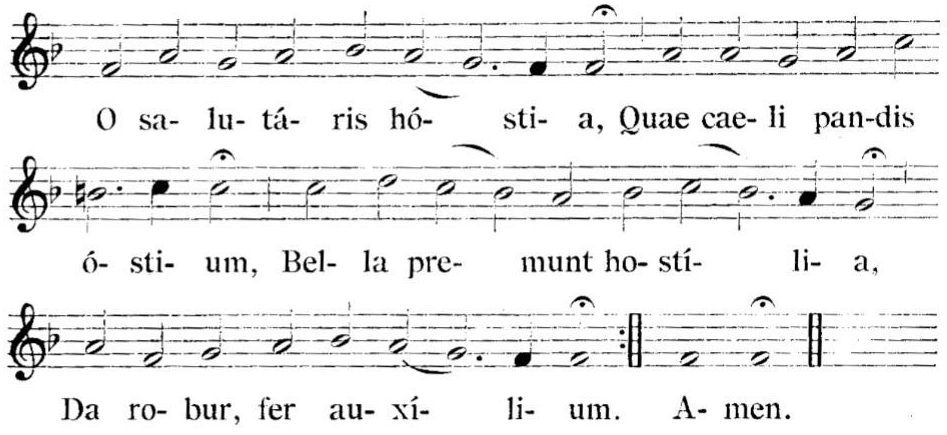
\includegraphics[width=\linewidth]{o-salutaris.jpg}
\end{figure}

\begin{center}
  \begin{footnotesize}
    \textit{
      Ô réconfortante
      Hostie, Qui nous
      ouvres les portes du
      ciel, les armées ennemies
      nous poursuivent,
      Donne-nous la force,
      porte-nous secours.
    }
  \end{footnotesize}
\end{center}

\begin{multicols}{2}
  \parindent=0pt
  \begin{flushright}
    O vere digna Hostia,\\
    Spes unica fidelium,\\
    In te confidit Francia,\\
    Da pacem, serva lilium.\\
  \end{flushright}
  \columnbreak
  \textit{
    Ô vraiment digne Hostie,\\
    Unique espoir des fidèles,\\
    en toi se confie la France,\\
    Donne-lui la paix, conserve le lys.\\
  }
\end{multicols}
\begin{multicols}{2}
  \begin{flushright}
    Uni trinoque Domino\\
    Sit sempiterna gloria :\\
    Qui vitam sine termino,\\
    Nobis donet in patria. Amen.\\
  \end{flushright}
  \columnbreak
  \textit{
    Au Seigneur unique en trois personnes,\\
    La gloire éternelle;\\
    qu'il nous donne en son Royaume\\
    La vie qui n'aura pas de fin. Amen\\
  }
\end{multicols}

\begin{center}
  \rule{2cm}{0.4pt}
\end{center}

\newpage

\begin{center}
  \textcolor{red}{\normalsize{En l'honneur de la Vierge Marie}}\\
  \textit{Voir au propre du jour}
\end{center}

\begin{center}
  \rule{2cm}{0.4pt}
\end{center}

\begin{center}
  \textcolor{red}{\normalsize{En l'honneur Du Saint Sacrement}}
\end{center}

\gresetinitiallines{1}
\greillumination{\initfamily\fontsize{11mm}{11mm}\selectfont T}
\gregorioscore{hy--tantum_ergo--solesmes}

\begin{multicols}{2}
  \parindent=0pt
  \textcolor{red}{\Vbar.} Panem de caelo praestitisti eis.\\
  \textcolor{red}{\Rbar.} Omne delectamentum in se habentem.\\
  
  \textit{\textcolor{red}{\Vbar.} Tu leur a donné le pain du ciel.\\
  \textcolor{red}{\Rbar.} Toute saveur se trouve en lui.}\\
  
\end{multicols}

\newpage

\begin{center}
  \textcolor{red}{\normalsize{Oraison}}
\end{center}

\begin{multicols}{2}
  \parindent=0pt
  Deus, qui nobis sub sacramento mirabili
  passionis tuæ memoriam reliquisti : \textcolor{red}{~†}
  tribue, quæsumus, ita nos Corporis et
  Sanguinis tui sacra mysteria venerari, \textcolor{red}{~*} ut
  redemptionis tuæ fructum in nobis
  jugiter sentiamus.\\
  Qui vivis et regnas
  cum Deo Patre in unitate Spiritus Sancti,
  Deus, per omnia sæcula sæculorum.
  Amen.
  \smallskip
  \columnbreak

  \textit{
    Seigneur Jésus Christ, dans cet admirable
    sacrement tu nous a laissé le mémorial de
    ta passion ; donne-nous de vénérer d’un si
    grand amour le mystère de ton Corps et de
    ton Sang, que nous puissions recueillir
    sans cesse le fruit de ta rédemption. Toi
    qui règnes avec le Père et le Saint Esprit
    pour les siècles des siècles.
    Amen. 
  }
\end{multicols}

\begin{center}
  \rule{2cm}{0.4pt}
\end{center}

\begin{center}
  \textcolor{red}{\normalsize{Louanges divines}}
\end{center}

\parindent=0pt
Dieu soit béni.\\
Béni soit son Saint Nom.\\
Béni soit Jésus-Christ, vrai Dieu et vrai homme.\\
Béni soit le Nom de Jésus.\\
Béni soit son Sacré Cœur.\\
Béni soit son précieux Sang.\\
Béni soit Jésus dans le très Saint Sacrement de l’autel.\\
Béni soit l’Esprit Saint Consolateur.\\
Bénie soit l’auguste Mère de Dieu, la très Sainte Vierge Marie.\\
Bénie soit sa Sainte et Immaculée Conception.\\
Bénie soit sa glorieuse Assomption.\\
Béni soit le nom de Marie, Vierge et Mère.\\
Béni soit Saint Joseph, son très chaste époux.\\
Béni soit Dieu dans ses anges et dans ses saints.\\
Seigneur, donnez-nous des prêtres.\\
Seigneur, donnez-nous de saints prêtres.\\
Seigneur, donnez-nous beaucoup de saints prêtres.\\
Seigneur, donnez-nous beaucoup de saintes vocations religieuses.\\

\begin{center}
  \rule{2cm}{0.4pt}
\end{center}

\newpage

\begin{center}
  \textcolor{red}{\normalsize{Déposition}}\\
  \textit{Psaume 116}
\end{center}

\gresetinitiallines{1}
\greillumination{\initfamily\fontsize{11mm}{11mm}\selectfont L}
\gregorioscore{ps--laudate_dominum_omnes_gentes_(psalmus_116)--solesmes}
\bigskip
\begin{footnotesize}
  \textit{
    Louez le Seigneur, tous les
    peuples ;
    Fêtez-Le, tous les pays !
    Son Amour envers nous
    S'est montré le plus fort ;
    Eternelle est la Fidélité du
    Seigneur !
    Gloire au Père, au Fils
    Et au Saint-Esprit,
    Comme il était au
    commencement,
    Maintenant et toujours,
    Pour les siècles des siècles,
    amen.
  }
\end{footnotesize}

\newpage

\begin{titlepage}\centering
  \vspace*{\fill}
  \LARGE Propre du temps.
  \vspace*{\fill}
\end{titlepage}

\newpage

\subfile{propre-epiphanie.tex}
\newpage
\subfile{septuagesime.tex}

\end{document}
